\documentclass[b5paper,zihao=-4]{ctexbook}
\usepackage{bigfoot}
	
\let\cleardoublepage\clearpage%去掉新开章节必须在右侧的限制

%以下内容是为了实现中式注释
%开始
\makeatletter
% 无上标的 \@makefnmark
\def\nosuper@makefnmark{\hbox{\normalfont\@thefnmark\space}}
% 补丁
\usepackage{etoolbox}
\patchcmd\@makefntext{\@makefnmark}{\nosuper@makefnmark}{}{}
\usepackage{xunicode-addon}
\newfontfamily\fnmarkfont{ipam.ttf}
\renewcommand\thefootnote{\hspace{-0.1em}{\footnotesize\fnmarkfont\textcircled{\arabic{footnote}}}}
\makeatother
%结束

\setCJKmainfont[BoldFont=方正准雅宋_GBK]{方正书宋_GBK}\setCJKmainfont[BoldFont=方正准雅宋_GBK]{方正书宋_GBK}
\setmainfont{Times New Roman}


\usepackage[left=1.27cm,right=1.27cm,top=2cm,bottom=2cm]{geometry}

\usepackage{titlesec}
	\assignpagestyle{\chapter}{fancy}
	
\usepackage{zhnumber}

\usepackage{xpinyin}
	%\xpinyinsetup{font={\fontspec{印氪先生汉语拼音 人教版W4}}}
	\xpinyinsetup{font={\fontspec{GB Pinyinok-B.ttf}}}

\usepackage{graphicx}

\usepackage{amsmath,caption}

\usepackage{indentfirst}

\usepackage{fancyhdr}
	\pagestyle{fancy}
	\fancyhf{}
	\fancyhead[RO]{\rightmark}
	\fancyhead[LE]{\rightmark}
	\fancyfoot[LE,RO]{\zhdigits{\arabic{page}}}
	\fancyhead[CO,CE]{\hyperref[mulu]{過子}}
	\renewcommand{\headrulewidth}{0.1mm}
	\renewcommand{\footrulewidth}{0mm}

\usepackage{xcolor}
	\definecolor{titlecolor}{RGB}{176,108,92}
	%\definecolor{titlecolor}{RGB}{0,0,0}

\usepackage{titletoc}
\contentsmargin{2em}
\titlecontents{chapter}% <section-type>
[2em]% <left> 距离左边界的距离
{\bfseries\large\linespread{2.0}\selectfont}% <above-code> 附加代码，比如字体大小等
{\thecontentslabel}% <numbered-entry-format> 隐藏编号
{}% <numberless-entry-format> 非编号项格式
{\dotfill\zhdigits{\thecontentspage}\hspace{3.8em}}% <fill-page-format> 点线和页码格式

\usepackage{pdfpages}

\usepackage[bookmarksopen,pdftitle=过子,hidelinks]{hyperref}

\renewcommand{\fangsong}{\CJKfontspec{方正仿宋_GBK}}
\renewcommand{\kaishu}{\CJKfontspec{方正楷体_GBK}}


\title{\hyperref[mulu]{\textbf{\fontsize{50}{50}過子}}}
\date{}
\author{\huge 依师过文氏教习之言辑}

\newcommand{\zhushi}[2]{#1 \footnote{〔#1〕#2}}
\newcommand{\zhushipy}[3]{#1 \footnote{〔#2〕#3}}

\begin{document}
%\begin{pinyinscope}
\linespread{1.3}\selectfont

\maketitle

\pagestyle{empty}\newpage\mbox{}\newpage

\frontmatter
\pagestyle{fancy}
\chapter*{序}

夫《过子》者，载圣人之言也。昔者化道既衰，礼乐崩坏，诸侯争雄，士风日下。然于斯时，有圣人过文氏出焉，名学，字登，号国文先生，华国人也。其生平以恢复化道为己任，倡逆等动定变之教，弟子两人，贤者二者有一。我等门人录其言行，集而成书，是谓《过子》。

观《过子》者，可以知元素之反应、实验之要义、有机之机理。凡读是书者，当慎思明辨，身体力行，庶几近道矣。

是以，《过子》乃化家经典之所宗，且华国文明之精髓。愿天下学子皆能通习之，取智其中，以期成为君子，共襄盛世之治，方不负吾师之志也。

\chapter*{前言}

自古以来，圣贤之言犹如明灯，照亮了无数寻求真理与智慧之路。过子，这位伟大的思想家、教育家，其生平言行不仅影响了他所处的时代，更穿越千年，成为后世治学修身的指南。在过子成名之后，作为他的弟子以及再传弟子们，他们深感责任重大，不敢让老师的教诲随风而逝。于是，他们将平日里聆听先生教导时记下的笔记，以及同门之间交流学习的内容整理成书，这就是《过子》。

本书汇集了过子关于逆等动定变、浮熔游响红等多方面的见解，通过简短精炼的语言表达了深刻的思想内涵。它不仅仅是一部记录过子言行的作品，更是foe文明宝库中不可或缺的一部分，承载着foe民族最宝贵的精神财富。

编辑整理过程中，为了保证其可靠性与真实性，我们将原文与著名写实文学《冼星海纪念中学闭路电视资料》进行校对，力求没有错漏。每当我们回顾这些文字时，都仿佛再次置身于那个充满智慧光芒的时代，感受到先师那温暖而又坚定的力量。希望这部作品能够让读者从中获得启发，无论是对于个人品德修养还是社会和谐发展都能有所裨益。

愿《过子》中的智慧之光永远照耀着人类前行的道路，指引我们向着更加美好的未来迈进。

庚子年秋，后学某某敬撰。

\tableofcontents
\label{mulu}

\titleformat{\chapter}{\centering\normalfont\huge\bfseries\color{titlecolor}}{}{0pt}{}
\mainmatter
\chapter[休息]{休息\protect\color[RGB]{0,0,0}\raisebox{0.3em}{\footnotemark}}
\footnotetext{据《冼星海纪念中学闭路电视资料》编。书中题目都是编者加的。}

昔者，磷烯与朗神课罢，相与弈于\zhushipy{庑}{庑（\pinyin{wu3}）}{指堂屋四周的小屋。}下。磷烯每举棋而疑，久之始落，故迨再上课时，局犹未竟。是时也，子过子巡至，睹其状，愠色\zhushipy{遽}{遽（\pinyin{ju4}）}{急速地。}现，曰：“\zhushi{吾观汝曹，岂需此多休耶？}{意思是，我觉得同学们不需要这么多休息时间！汝曹，你们，曹，辈，相当于“们”。}夫学者，当以学为重，争分夺秒。今溺于棋戏，忘却时辰，非所宜也！”

先生言讫，左右皆默，悟其教诲之深意，遂各返其位，整衣待课。子过子复前行，视他处。

\chapter{拖课}

昔者，子过子于堂上讲学，时近午刻，诸生皆饥肠辘辘。将下课之际，硼氢锂者，坐于后门之旁，悄启其扉，欲俟课毕即趋食堂。是时也，子过子察焉，怒而叱曰：“速阖尔扉！\zhushi{若复有分心之举，吾必延课十刻！}{意思是，你要是再这样，我就拖课十分钟！}”闻此言，满座皆惊，旋而哄堂大笑。

于是，诸生虽饿，然感夫子训诫之重，不敢稍懈。硼氢锂闻命，遽闭后门，众皆敛容正坐，复听夫子讲解。斯事既彰子过子治学之严，又见师生和乐之情状。课堂之上，虽偶有嬉闹，终不失规矩，实乃教学相长之美事也。

\chapter{狼叫}

昔者，子过子于实验课授诸生以滴定管之用。器虽微，然于化道实验至重，非心静手稳者不能得其妙。是日也，堂上喧哗四起，锂钼锶数人尤甚，高声呼叫，嬉戏不休，以致子过子之言几不可闻。

见此状，子过子止其讲，面有愠色，厉声道：“\zhushi{尔等勿为狼叫！}{意思是，不要狼叫！}课堂者，求学之所；非市井游乐之地。今吾所授，关乎尔等学问之基，岂可轻慢？若真心向学，当敛神静听；若仍肆意妄为，乱吾课堂，则必罚之，以肃学风。”

锂钼锶等闻此言，皆惭而默，知其行有失。遂敛容收声，专心致志，静听子过子续讲。其余学子亦随之安静，堂复归肃穆。子过子见状，乃再提滴定管，细述其用，诸生皆凝神倾听，受益匪浅。
\chapter{捅刀}

昔者，子过子之于弟子也，犹父之于子，未尝不教诲而期望焉。或有弟子，非礼而议其师，此言终闻于子过子耳，子过子忿然曰：“吾之所恶，莫大于人之背施奸计，口蜜腹剑。\footnote{〔吾之所恶……口蜜腹剑。〕意思是，我最讨厌别人在我背后捅刀子。}夫君子立身行事，当光明磊落，今见此行，吾心痛矣。”

“吾闻有言：‘吾不能善教。’此言如刃刺吾之心，令吾痛不可忍。”子过子立堂上而言，“为人师者，岂敢懈怠？每思及汝等学业，无不殚精竭虑，夙夜忧叹。若真有所不足，愿尔等直言无讳，而非私语诽谤。盖诚言利于改进，暗箭伤人，徒增怨恨。”

“古之君子，忠信为本。今有人背地非议，实为不忠不信之举。吾虽不才，亦求诸生于堂上以诚相待，毋使奸佞之风染于学堂。《诗》云：‘靡不有初，鲜克有终。’学者之初，皆怀敬意；及其久也，或生厌倦。然师生之间，犹父子兄弟，当相敬相爱，何至于此？”

“且教育之事，需时日积累，方能见成效。古之贤者，无不由勤奋而来，岂有懒惰而成大器者乎？今诸生\zhushipy{评骘}{评骘（\pinyin{zhi4}）}{评定高低。}，原为共进，非为攻\zhushipy{讦}{讦（\pinyin{jie2}）}{攻击别人的短处。}。若有不满，当面陈说，共商良策，岂不美哉？愿诸君深思吾言，勿忘初心，共勉之。”

\chapter{免疫}

季冬岁暮，诸生赴试，守旧难展。子过子览卷毕，色凝重，训曰：“汝等于业，其有免疫之功耶？”长叹悲来，\zhushi{心凉}{据《冼星海纪念中学闭路电视资料》载，当时原话是“我心中只有两个字：凉凉。”}。晨兴夜寐，讲圣贤道，今得此报，心寒。

硼氢锂欲往他室自习，为子过子所止。子过子立堂前，曰：“考绩不佳，今欲何往？”

硼氢锂驻步答：“觅静处补业。”

子过子摇头叹曰：“非也，汝之缺者，课堂未尽心也。若汝一心向学，则不致今日境地。”又正色道：“听课不专，策试难如意。今后改弦更张，莫负光阴恩情。留于此，随我修习，或可补救。”

硼氢锂闻之愧疚，应诺归位，决心专心，不敢懈怠。

\chapter{火星}

子过子观诸生课业测验之成绩，见其多不尽如人意，心中愤懑，乃厉声而言曰：“观汝等所获分数，几使我怒火中烧，头上似有火星迸发！\footnote{〔观汝等……火星迸发！〕意思是，我看你们这个成绩，我头上都要冒火星子了。}”

于是时也，讲堂之内寂然无声。子过子面若寒星，继而责之曰：“尔等日受吾教，今竟至此，岂不痛心疾首？”

复言曰：“学识之事，犹筑城者，需砖石稳固，不可有懈怠。今汝等所为，恰城墙未固，风雨骤至，岂能无恙？吾日夜操劳，竭力传道授业，正望汝等有所成。然今日视之，实令吾失望。”

众弟子闻此，皆垂首默然。

\chapter{保送}

化学之堂，诸生皆正襟危坐，凝神静听夫子讲授化学幽微之理。时也，子过子忽而转目，见弟子紫外线者，不顾化学之课，奋笔疾书于数学竞赛之卷，遂面有愠色，\zhushipy{蹙}{蹙（\pinyin{cu4}）}{皱（眉）。}眉瞋目，厉声责之曰：“\zhushi{汝竟欲保送乎？}{是不是要保送了？}当此化学授业之时，心却游移，此非求学之道也！”

夫师者，传道、授业、解惑之人也；见弟子分心，则即刻警醒之，愿其明学业需专精，不可二心。此亦显师徒之间情谊深厚，相互督责，共勉学问真谛。紫外线闻师训，应深思己过，专意化学，他日或能双科并进，不负师望。如此师生相与，实为教化之美谈。
\chapter{宣科}

夫子过子，评骘\zhushipy{庠序}{庠（\pinyin{xiang2}）序}{学校。}之风，喟然叹曰：“今之师者，若\zhushi{唯诵书本而不通变}{据《冼星海纪念中学闭路电视资料》载，原话是“一个老师如果只会照本宣科，那他就不是一个好老师。”}，则非良师也。”其意讽喻当世教者，徒守旧章，鲜启迪心智之能。而子过子治学，谨严备至，临讲席之前，必考究学问真伪，核对典籍，以求无误。彼以为传道授业，解惑为重，未尝轻言书外之事。是以学者得遇此君，如沐春风，心悦诚服，皆因其言必信，行必果，实为后学之楷模。

\chapter{狂笑}

夫子过子亲授尻佬拭窗之法。\zhushi{维}{起强调作用，无实义。}时秋暮，光影交错。子过子指窗台尘埃之处，状若戏谑，千焓见之，忍俊不禁，群笑随之。子过子愕然，厉色责曰：“吾何所言，致尔等狂笑？\footnote{〔吾……狂笑？〕意思是，我说了什么，让你狂笑不止？}”千焓正色答曰：“非敢轻慢，适见师以手势示尘，其态可掬，是以失笑。”众闻其言，皆释然，一时笑声盈室。子过子亦霁颜悦色，续其教导，心自许曰：“往后授课，当慎择言行，以免再生误解。”自是之后，师生之间默契日深，欢愉愈增。
\chapter{清除}

硼氢锂者，因前夜迟眠，翌日授课之时，昏昏欲寐，慵懒之状甚著。子过子屡次警示，终忍无可忍，遽厉声叱曰：“\zhushi{汝若无意于学，吾将黜汝于门外！}{意思是，不想学，你就给我滚出去！}”硼氢锂闻之，赧然无地自容，愧悔交集，不敢复有懈怠。

迨课毕，子过子未尝记其咎，反慈颜温语诫之曰：“\zhushi{嗣后}{从此以后。嗣，从此。}必善自调摄，早卧早起，以养精神，庶几能致志于学。”硼氢锂听罢，心悦诚服，拜谢师恩，誓改前非，再不重犯。自此之后，每临讲堂，皆神采奕奕，勤勉向学，师生之间情谊益厚。

\chapter{投掷}

上课之刻，曾孙者，潜阅报章，未虞为子过子所察。子过子，师也，见状心愠，遂悄然而至其后。俄而夺其报，掷诸室外，面有怒色而言曰：“尔母每询吾，何以汝学绩不佳，自今勿复使汝母问吾何以汝学业之劣，不然，吾将以此事告之\footnote{〔自今……告之〕你以后不要让你妈再来问我为什么你的成绩这么差，不然我就把这件事告诉她。}。”

且夫曾孙，出自望族，当承祖训，励志向学，岂可分心于杂书哉？子过子诫之，亦望其改过自新，专心致志于学业，勿负家族厚望。曾孙闻此，惭愧难当，诺诺而应，誓不再犯，愿自此奋发图强，以慰长辈之期许。

\chapter{恍惚}

上课之刻，子过子见$\overrightarrow{\text{向量}}$私撰\zhushi{悟净}{据《冼星海纪念中学闭路电视资料》载，方言，即全国中学\underline{生物}\hspace{-0.05em}理竞赛。}之题，心弗悦。遂厉声责曰：“吾观汝似愈学愈迷，神思恍惚矣。若再为吾所见，必\zhushi{碎汝卷}{把试卷撕得稀巴烂。}，令无复阅！”

夫$\overrightarrow{\text{向量}}$者，颖悟之士也，然于课上分心，非正途矣。子过子诫之，意在使其明轻重、守\zhushipy{矩矱}{矩矱（\pinyin{yue1}）}{法度。}，专于当务之学。

$\overrightarrow{\text{向量}}$闻师言，赧然而惭，诺而应允，誓不再犯。自是之后，每遇难题，皆俟课余方思，不敢再于堂上驰骛。

且夫学问之道，在乎专一。$\overrightarrow{\text{向量}}$既欲竞赛，亦当择时而动，不可因一时之兴，误正业。子过子之言，虽严苛，实出于关爱之心，望其能明事理，有所成也。

\chapter{笔记}

子过子授化学，见铁锂子凝神执笔，疑私习题，色厉问之：“\zhushi{汝今何为？}{意思是，你在写什么？为，做，这里有“写”的意思。}”铁锂子惊对：“记先生所授。”子过子察之，知误，心愧。

教学之间，沟通为要。子过子未详察，致误会，幸明真相，免屈良材。铁锂子专学不愠，亦学子楷模也。事示吾等，行当审慎，勿错判人意，伤和气。师生之情，贵于信任，方可共进学业。

\chapter{煮面}

昔者，日入而暝，诸生腹馁，窃于庠序之中\zhushipy{爨}{爨（\pinyin{cuan4}）}{生火做饭。}汤煮\zhushipy{麪}{麪（\pinyin{mian4}）}{“面”的繁体字“麺”的异体字。}以充饥。初，子过子遇之，未尝怒也，乃诲之曰：“汝等宜俟课毕而后食。”然数秒之后，复见有生私爨，子过子忿然而言曰：“\zhushi{凡不志于学者，今可去矣！}{不想学，现在就可以离开！}”

子过子虑此行渐成弊俗，伤及教化之本，故严辞以诫，欲使诸生知礼守义，重学修身。时夜已深，灯火荧荧，众弟子闻其言，皆默而不语，若有所思。子过子又进而言曰：“夫学者，所以明德、亲民、止于至善也。毋以小欲害大道。”

\chapter{乘车}

昔者，子过子与诸弟子行于郊野。途遥路险，皆徒步而进。然则子过子心急欲速达，遂独乘一车，冀其隐。至中途，忽一弟子惊曰：“夫子之步数寡矣，似有乘车之迹。”子过子闻之，正色而言曰：“\zhushi{吾岂乘车者？此乃尔等误也。}{诶？我没有骑车啊？你们看错了！}”其言甚坚，不容置疑。

时有一老成弟子出列，揖而问曰：“夫子，同道而行，何故公之足印稀疏，且面无劳色？”子过子笑曰：“吾守礼义，未尝为私利变节。尔等所见，必他车之痕，非吾乘也。”

众弟子虽心存疑虑，然见师态度凛然，不敢复言。此事遂成私下议论，终未敢再问。子过子以身作“则”，意在示教，使弟子知诚信与守礼之重。

\chapter{作业}

子过子为诸生市课业，名曰《一遍过》。一日，临堂察诸生作业，见十不存一，心甚忧之，乃厉色而言曰：“汝等虽好习竞赛，然不可忘却高考之要。”又叹曰：“有弟子不知天高地厚，若非自慎，则祸不远矣！\footnote{〔若非自慎，则祸不远矣！〕意思是，不作死，就不会死！}苟免考而入高等学府者，吾亦乐见其成，此非徒言也。\footnote{〔苟免考……此非徒言也。〕据《冼星海纪念中学闭路电视资料》载，当时原话是“如果你们真的能够保送，I'm proud of you!”}”

子过子言时，声色俱厉，目光如炬，巡睃四座，似有不尽期许之意。众弟子闻之，皆垂首无语，面有愧色，心知其咎，不敢再怠。一时之间，室内静默无声，唯闻子过子教诲之音。诸生受此激励，咸立志改过自新，勤勉向学，以不负师恩。

\chapter{谈话}

昔有一生，名曰木雨，其人聪慧伶俐，于诸学科皆有建树。一日，化道课业成，然其绩却未如人意，子过子闻之，心忧此子未能尽展所学，故召之至办公室，欲与其详谈。

木雨入室，见子过子面色凝重，知事不妙，遂敛容正坐。子过子徐展其成绩单，指上所书成绩，面有忧色而言：“汝观其余科目，皆能名列前茅，独化道一科，成绩稍逊。岂欲自承其不善乎？”木雨闻言，低头无语，心中暗自惭愧。

子过子见状，又言道：“非是汝不能也，乃不为耳！\footnote{〔非是……乃不为耳！〕意思是，不是你做不到，是你不想做！}吾闻汝好游戏，每下课必与同窗嬉戏，然则化道一门，实为科学之基石，关乎天地万物之理，若能深究，则趣味无穷矣。”

木雨听罢，感师之教诲，思己过失，遂立志改之。

\chapter{换字}

子过子素尚学风，见诸生有懈怠者，心忧之。择日，欲以辞激勉弟子，遂取墨笔，书“放手拼博，每分必争”八字于讲堂之前壁，期使入室者皆能目遇而奋发。

然子过子一时疏忽，“搏”字误作“博”。课间休息，诸生偶见此异，窃议纷纷。既知其误，不忍师长蒙羞，决意共襄义举。于是乎，群策群力，仿照原字之形，精心设计，终得一佳制。更选斑斓彩纸，令新字焕发光彩，与旧字无异，贴于壁上，宛如天生。

然则，锂钼锶午后自外归来，未知前事，乍见一字有异，心中顿生疑窦，步近前，欲窥究竟。子过子适逢其会，突现眼前，见锂钼锶举动，以为其戏谑，怒从心起，厉声责曰：“汝闲甚耶？若以此精力用诸学业，则何愁不成？\footnote{〔汝闲甚耶……何愁不成？〕又闲了是吧？要是你把这精力放在化竞上，比什么都强！}”锂钼锶惊，欲辩解，子过子已拂袖而去，误会未解。

自此，子过子每望此字，心有不甘；锂钼锶亦觉遗憾，未能释明己志。此事传开，众议纷纭，或叹师长督责之严，或赞同学相助之美德，唯憾误解未能得解也。

\chapter{指导}

一日，子过子授化学课，命诸生各自习业。时子过子巡班级，见木雨独坐其位，笔未尝动，遂前而导之。子过子详观其态，察其难处，语重心长，示以解惑之道。

及至考毕，子过子览木雨卷，见仅得五十分，不觉怒形于色，责曰：“何故仅此分数？汝之小脑瓜究作何思？\footnote{〔汝之小脑瓜究作何思？〕你的小脑 瓜子是做什么用的？}”木雨闻之，面有愧色，欲言又止，心中忐忑，未能即刻道破真相。盖木雨算分之际偶有差池，误将己分书为五十，非其真实所得也。然木雨素来好学，此次失误，实出无心，心内亦自责不已，惟恐师长误会，同窗见笑。子过子不知此中曲折，但见木雨默然不语，以为悔悟，乃叹一口气，冀其日后更进。

\chapter[过文]{过文\protect\color[RGB]{0,0,0}\raisebox{0.3em}{\footnotemark}}
\footnotetext{据《冼星海纪念中学闭路电视资料》载，“过文”为方言，意为一切球状物体，这里指弹力球。}

诸生课间无事，遂购得一过文于门外嬉戏。因子过子疏于督责，诸生渐放肆，乃自门外移至教室内后方玩乐，至自习之时亦复如是。球来球往，声震四壁，扰及左右。

一日入夜，教室灯火通明，而子过子办公室之灯已灭，众以为其已归家，心中大喜，愈加无所顾忌，喧哗之声更甚。游戏自下课始，至上课时犹未止息，仿若无人能制此乱局。

俄而，大硫正端坐于前，忽闻一声轻响，过文自背后飞来，恰中其头。大硫惊起，怒目圆睁，欲取球还掷，众见状，哄然作鸟兽散，唯恐避之不及。然未几，窗外忽现阴影，子过子面色铁青，双目似炬，视若猛虎出柙，令人心惊胆战。众皆噤声，不敢妄动。

大硫见势不妙，一边叱骂掷球之人，一边将手中之过文交与窗外之子过子。子过子接球在手，面有愠色，五指紧握，似鹰爪状，仿佛欲捏碎此球以泄愤，然球固且韧，未能如愿。遂仰首厉声道：“吾从未遇纪律如此之劣之化学竞赛班！\footnote{〔吾从未遇……化学竞赛班！〕我从没见过纪律这么差的化学竞赛班！}”

言罢，稍顿，复加严厉曰：“唯余两日！唯余两日，尔等便将散矣！\footnote{〔唯余两日……散矣！〕还有两天，还有两天，你们就要结束啦！}”

子过子言毕，即遂即转背，愤然远引，惟余众人呆立原地，面面相觑，心中各有所思。

\newpage
\vfill
\begin{figure}
	\centering
	\begin{minipage}{\textwidth}
		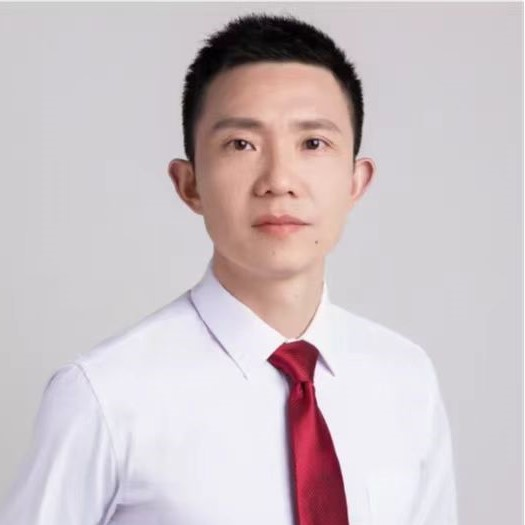
\includegraphics[width=\textwidth]{gwx.jpg}
	\end{minipage}
	\caption*{\normalsize\bfseries 过子像 \\ \footnotesize\normalfont\centering （来源：《冼星海纪念中学闭路电视资料》）}
\end{figure}
\vfill

\newpage
\pagestyle{fancy}
\chapter*{\color[RGB]{0,0,0}后记\\ \normalsize——为了过文的记念}
大抵是二零二五年一月四日的正午，我独坐在少科院那连打印机都没有钱买硒鼓却充满回忆的教室里，面前摊开着这篇《过子》。初时，不过是兴起，欲仿效《论语》之笔调，将吾家文学先生的些许场景描绘一番，博诸君一笑而已。未曾想，这一做起来，竟似有别样的意味在其中了。

从最初的《休息》，到后来着手编撰教科书，此事渐渐在我生活中占据了不小的分量。每日傍晚自习前的将近四十分钟，以及自习结束后那短短的二十多分钟，都成了我与《过子》相伴的时刻。要说这事情何以能引起我如此多的关注，实在难以言喻；然而，当得知此书即将付梓，分发至全班同学手中之时，心中难免泛起一丝小小的成就感来——虽则这种成就，在旁人看来或许微不足道。

然则，我虽不才，却也深知，作为一个尚未成型的竞赛生，不应在此事上耗费过多光阴。故而，即便将来还会有许多值得记录的名场面，《过子》大约也只能就此告一段落了罢。这并非不愿继续，但在不务正业了这么久之后，大抵也该干点正事了\footnote[1]{指玩第五人格？}。世间之事，往往如此，得失之间，总须有所权衡。

不是年青的为年老的写记念，而在这两年中，却使我目睹许多化竞的题，层层淤积起来，将我埋得不能呼吸，我只能用这样的\LaTeX，写几句文章，算是从泥土中挖一个小孔，自己延口残喘，这是怎样的世界呢。夜正长，路也正长，我不如藏住，不说的好罢。但我知道，即使不是我，将来总会有记起他，再谈他的时候\mbox{的……}
\begin{flushright}
	编者
	
	文沙路25号
	
	甲辰龙年腊月初五
\end{flushright}

%\end{pinyinscope}
\end{document}